
%% Based on the style files for ACL-IJCNLP-2009, which were, in turn,
%% based on the style files for EACL-2009 and IJCNLP-2008...

%% Based on the style files for EACL 2006 by 
%%e.agirre@ehu.es or Sergi.Balari@uab.es
%% and that of ACL 08 by Joakim Nivre and Noah Smith

\documentclass[11pt,letterpaper]{article}
\usepackage{naaclhlt2013}
\usepackage{times}
\usepackage{url}
\usepackage{latexsym}
%\usepackage{supertabular}
%\setlength\titlebox{6.5cm}    % You can expand the title box if you
% really have to
\usepackage{graphicx}
\usepackage{placeins}


\title{Sense or nonsense? Parameter optimisation for Cross-Lingual Word-Sense Disambiguation}

\author{Maarten van Gompel, Antal van den Bosch \\
  Centre for Language Studies \\
  Radboud University Nijmegen \\
  {\tt proycon@anaproy.nl}}

\date{}

\begin{document}
\maketitle
\begin{abstract}
We present our system WSD2 which participated in the Cross-Lingual Word-Sense Disambiguation task for SemEval 2013 \cite{TASKPAPER}. The system closely resembles our winning system for SemEval 2010 and is based on k-nearest neighbour classifiers which map words with local and/or global context features onto their translation, i.e cross-lingual sense. The system participates for all five languages in the task and obtained winning scores for four of them when asked to predict the best translation(s). We tested various configurations of our system, focusing on various levels of parameter optimisation. 
\end{abstract}


\section{Introduction}

WSD2 is a rewrite and extension of our previous system \cite{WSD1} that participated in the Cross-Lingual Word Sense Disambiguation task in SemEval 2010. In WSD2 we introduce and test a new level of parameter optimisation and unlike before we participare for all five target languages (Dutch, Spanish, Italian, French, German). The task presents twenty nouns with fifty instances each to be disambiguated. The instances consist of a form of the noun in the context of a single English sentence. This word is to be translated into the five target languages. The sense of the word we predict is thus its translation given a certain context. The translations/senses in all cases are uninflected lemmas. Trial data is provided and has been used to optimise system parameters. Due to the unsupervised nature of the task, no training data is provided. However, given that the gold standard of the task is based exclusively on the Europarl parallel corpus \cite{Europarl}, we select that same corpus to minimise our chances of delivering translations that the human annotators preparing the test data could have never picked.
   
The system may output several senses per instance, rather than producing just one sense prediction. These are evaluated in two different ways. The scoring type ``\textbf{best}'' expects that the system outputs the best senses, in the order of its confidence. Multiple guesses are penalised. The scoring type ``\textbf{out of five}'' expects five guesses, in which each answer carries the same weight. These metrics are more extensively described in \cite{CLLS} and \cite{TASKPAPER}. 

\section{System Description}

The WSD2 system, like its predecessor, makes use of word experts. Each word expert is a $k$-nearest neighbour classifier specialising in the disambiguation of a single of the twenty provided nouns. This is implemented using the Tilburg Memory Based Learner (TiMBL) \cite{TIMBL}. The classifiers are trained as follows: First the parallel corpus which acts as training data is tokenised using Ucto \cite{UCTO}, for all five language pairs. Then, a word-alignment between sentence pairs in the Europarl training data needs to be established, for which we use GIZA++ \cite{GIZA}. We use the intersection of both translation directions, as we know the sense repository from which the human annotators preparing the task's test data can select their translations is created in the same fashion. 

Whereas the word alignment is computed on the actual word forms, we also need lemmas for both the source language (English) as well as all of the five target languages, because the English nouns in the test data can be either singular or plural. The target translations all have to be lemmas, so variation in gender, number and/or case is not maintained. Moreover, to be certain we are dealing with nouns in the source language, a Part-of-Speech tagger is also required. Part-of-Speech tagging and lemmatisation is conducted using several tools depending on the language. Freeling \cite{FREELING} was used for English, Spanish and Italian, Frog \cite{TADPOLE} for Dutch, and TreeTagger \cite{TREETAGGER} for German and French. 

With all of this data generated, we can subsequently iterate over all sentences in the training data and extract occurrences of any of the twenty nouns, along with the translation they are aligned to (if any). We extract the words themselves, the lemma, the part-of-speech tag and do the same for a specified number of words to the left and to the right of the found occurrence. These constitute the local context features. In addition to this, global context features are extracted; these are a set of keywords per lemma and per translation which are repeatedly found at arbitrary positions in the same sentence. 

The global context features are represented as a binary bag-of-words model in which the presence of each of the keywords that \emph{may} be indicative for a given word to sense/translation is represented by a boolean value. Such a set of keywords is constructed for each of the twenty nouns, per language. The scope in whcih keywords are extract is one sentence, as this is the widest context supplied in the test data.

%<very close paraphrase from earlier paper>
The method used to extract these keywords ($k$) is proposed by \cite{NgL96} and used also in the research of \cite{Hoste+02}. Assume we have a focus word $f$, more precisely, a lemma of one of the target nouns. We also have one of its aligned translations/senses $s$, also a lemma. We can now estimate $P(s|k)$, the probability of sense $s$, given a keyword $k$, by dividing $N_{s,k_{local}.}$ (the number of occurrences of a possible local context word $k$ with particular focus word lemma-PoS combination and with a particular sense $s$) by $N_{k_{local}}$ (the number of occurrences of a possible local context keyword $k_{loc}$ with a particular focus word-PoS combination regardless of its sense). If we also take into account the frequency of a possible keyword $k$ in the complete training corpus ($N_{k_{corpus}}$), we get:

\begin{equation}
P(s|k) = \frac{N_{s,k_{local}}}{N_{k_{local}}}(\frac{1}{N_{k_{corpus}}})
\end{equation}

\cite{Hoste+02} select a keyword $k$ for inclusion in the bag-of-words representation if that keyword occurs more than $T_1$ times in that sense $s$, and if $P(s|k) \ge T_2$. Both $T_1$ and $T_2$ are predefined thresholds, which by default were set to $3$ and $0.001$ respectively. In addition, WSD2 and its predecessor WSD1 contain an extra parameter which can be enabled to automatically adjust the $T_1$ threshold when it yields too many or too few keywords. The selection of bag-of-word features is computed prior to the extraction of the training instances, as this information is a prerequisite for the successful generation of both training and test instances. 
%</very close paraphrase from earlier paper> 

\section{Parameter Optimisation}

The size of the local context, inclusion of global context features and inclusion of syntactic features are all parameters to the system. These allow for a variety of combinations to be tested. In addition, each word expert is a k-nn classifier that can take on a myriad of parameters. In this study we decided to focus on various levels of parameters optimisation. One level of parameter optimisation includes the optimisation of the classifier parameters for each of the word experts, these are optimised on the training data and evaluated through cross-validation. The parameter search algorithm \cite{PARAMSEARCH} was used here. Whereever parameter search was not used, we used a value of $1$ for $k$ and default values for all other parameters to Timbl.

A development set for the twenty nouns has been made available by the task organisers; this allows for further optimisation. We decided to test various parameters to the system, combined with the optimisation of classifier parameters as described above and per word-expert select the one with the highest score on the development set. This is done seperately for both evaluation metrics in the task.

\section{Experiments \& Results}

To assess the accuracy of a certain configuration of our system as a whole, we take the average over all word experts. An initial experiment on the \emph{trial data} explores the impact of different context sizes, with parameter optimisations on the classifiers. The results, shown in Figure~\ref{figcontext}, clearly indicate that on average the classifiers perform best with a context-size of just one word; meaning one word to the left and one to the right of the word to be disambiguated. Larger context sizes have a negative impact on average accuracy. Selective analysis has shown this same trend to hold if parameter optimisation is not performed.

\begin{figure}
\label{figcontext}
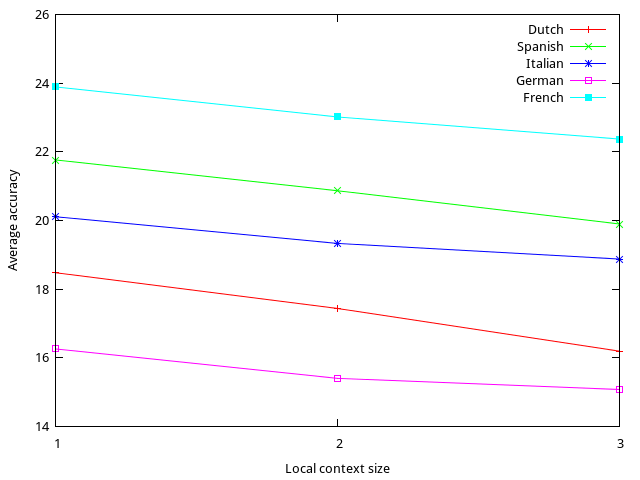
\includegraphics[width=8cm]{context.png}
\caption{Average Accuracy for different local context sizes}
\end{figure}

We submitted three configurations of our system, the maximum, to the shared task. Adding lemma features on average proves beneficial, as shown in the Table~\ref{tabtrialresults}. This is therefore the first configuration we submitted (\texttt{c1l}), as second configuration (\texttt{c1lN}) we submitted this same configuration without parameter optimisation on the classifiers.

\begin{table}
\footnotesize
\label{tabtrialresults}
\begin{tabular}{|l|r|r|r|r|r|}
\hline
\textbf{BEST} & \textbf{ES} & \textbf{FR} & \textbf{IT} & \textbf{NL} & \textbf{DE} \\
\hline
baseline &  19.65 & 21.23 & 15.17 & 15.75 & 13.16 \\
\hline
plain & 21.76 & 23.89 & 20.10 & 18.47 & 16.25 \\
$+$lem (\texttt{c1l}) & 21.88 & \textbf{23.93} & \textbf{19.90} & \textbf{18.61} & \textbf{16.43} \\
$+$pos & 22.09 & 23.91 & 19.95 & 18.02 & 15.37 \\
lem$+$pos & \textbf{22.12} & 23.61 & 19.82 & 18.18 & 15.48 \\
\hline
glob.context & 20.57 & 23.34 & 17.76 & 17.06 & 16.05 \\
\hline
\textbf{OUT-OF-5} & \textbf{ES} & \textbf{FR} & \textbf{IT} & \textbf{NL} & \textbf{DE} \\
\hline
baseline & 48.34 & 45.99 & 34.51 & 38.59 & 32.90 \\
\hline
plain & 49.81 & \textbf{50.91} & 42.30 & 41.74 & \textbf{36.86} \\
$+$lem (\texttt{c1l}) & \textbf{49.91} & 50.65 & \textbf{42.41} & \textbf{41.83} & 36.45 \\
$+$pos & 47.86 & 49.72 & 41.91 & 41.31 & 35.93 \\
lem$+$pos & 47.90 & 49.75 & 41.49 & 41.31 & 35.80 \\
\hline
glob.ccontext & 48.09 & 49.68 & 40.87 & 37.70 & 34.47 \\
\hline
\end{tabular}
\caption{Feature exploration on the development set}
\end{table}

The third configuration (\texttt{var}) we submitted selects \emph{per word expert} the configuration (always with parameter optimisation on the classifier) that has the highest score on the development set, and thus mixes all kinds of configurations and by definition leads to the highest scores on the development set, with the risk of overfitting. Results on the development set are shown in Table~\ref{tabpar}.

\begin{table}
\footnotesize
\label{tabpar}
\begin{tabular}{|l|r|r|r|r|r|}
\hline
\textbf{BEST} & \textbf{ES} & \textbf{FR} & \textbf{IT} & \textbf{NL} & \textbf{DE} \\
\hline
c1lN & 22.60  & 24.09 & 19.87 & 18.70 & 16.43 \\ 
c1l & 21.88 & 23.93 & 19.90 & 18.61 & 16.43 \\ 
var & 23.79 & \textbf{25.66} & \textbf{21.65} & \textbf{20.19} & \textbf{19.06} \\
varN & \textbf{23.90} &  25.65 & 21.52 & 19.92 & 18.96 \\ 
\hline
\textbf{OUT-OF-5} &  \textbf{ES} & \textbf{FR} & \textbf{IT} & \textbf{NL} & \textbf{DE} \\
\hline
c1lN & 50.14 & 50.98 & 42.92 & 42.08 &  36.45 \\
c1l & 49.91 & 50.65 & 42.41 & 41.83 & 36.45 \\ 
var & 51.95 & \textbf{53.66} & 45.59 & \textbf{44.66} & \textbf{39.81} \\
varN & \textbf{52.91} & 53.61 & \textbf{45.92} & 44.32 & 39.40 \\
\hline
\end{tabular}
\caption{Results on the development set}
\end{table}
 
The parameter optimisation on training data, optimised on classifier accuracy, has a slight negative impact. Therefore a fourth configuration (\texttt{varN}) was tried later to independently assess the idea of variable configuration selection, without parameter optimisation on the classifier. This fourth configuration however was not yet available for the actual competition, but this incidentally would have had no impact on the final ranking between competitors anyway. When we run these systems on the actual test data of the shared task, we obtain the results in Table~\ref{tabfinal}. The best score amongst the other competitors is mentioned for reference.

\begin{table*}[tb]
\footnotesize
\label{tabfinal}
\begin{center}
\begin{tabular}{|l|r|r|r|r|r|}
\hline
\textbf{BEST} & \textbf{Spanish} & \textbf{French} & \textbf{Italian} & \textbf{Dutch} & \textbf{German} \\
\hline
c1l &  28.40 & 29.88 & 25.43 & 23.14 & 20.70 \\
c1lN &  28.65 & 30.11 & \textbf{25.66} & \textbf{23.61} & 20.82 \\
var & 23.3 & 25.89 & 20.38 & 17.17 & 16.2 \\
varN & 29.05 & \textbf{30.15} & 24.90 & 23.57 & \textbf{21.98} \\
best competitor & \textbf{32.16} (Marine) & 28.23 (alexr) & 24.62 (alexr) & 22.36 (alexr) & 19.92 (alexr) \\ 
\hline
\textbf{OUT-OF-FIVE} & \textbf{Spanish} & \textbf{French} & \textbf{Italian} & \textbf{Dutch} & \textbf{German} \\
\hline
c1l &  58.23 & 59.07 & 52.22 & \textbf{47.83} & 43.17 \\
c1lN & 57.62 & \textbf{59.80} & 52.73 & 47.62 & 43.24 \\
var & 55.70 & 59.19 & 51.18 & 46.85 & 41.46 \\
varN & 58.61 & 59.26 & 50.89 & 50.42 & 43.34 \\
best competitor & \textbf{61.69} (alexr) & 58.20 (alexr) & \textbf{53.57} (alexr) & 46.55 (alexr) & \textbf{43.66} (alexr) \\ 
\hline
\end{tabular}
\end{center}
\caption{Results on the test set}
\end{table*}

A major factor in this task is correct lemmatisation, and to far lesser extent, part-of-speech tagging. We conducted some additional experiments on German and French without lemmatisation, tested on on the development data. Results immediately fell below baseline. 

Another main factor is the quality of the word alignments, and the degree to which the found word alignments correspond with the translations the human annotators could choose from in preparing the gold standard. An idea we tested is, instead of relying on the mere intersection of word alignments, to use a phrase-translation table generated by and for the Statistical Machine Translation system Moses, which uses the grow-diag-final heuristic to extract phrase pairs. This results in more phrases, and whilst this is a good idea for MT, in the current task it has a clear detrimental effect, as it creates too many translation options and we do not have an MT decoder to discard ineffective options in this task. The grow-diag-final heuristic tends to incorporate unaligned words to the end of a translation in the translation option, which for our purposes is a bad idea.

\section{Conclusion}

In this study we have taken parameter optimisation one step further compared to our previous research \cite{WSD1}; by using a variable selection of system parameters from the best configurations on the development data. This idea proves to have a slight edge. Parameter optimisation of the classifiers on the training data however, proves to have a slightly negative effect, especially when combined with the selection of variable configurations. This clearly suggests overfitting. 

We can furthermore uphold the conclusion from previous research that including lemma features is generally a good idea. As to the number of local context features, we conclude that a context size of one feature to the left, and one to the right, has the best overall average accuracy. In fact, due to our variable configuration selection without parameter optimisation on the classifier not being available yet in the contest, our simplest system \texttt{c1lN} emerged as best in the contest.

When asked to predict the best translation(s), our system comes out on top for four out of five languages; only for Spanish we are surpassed by two competitors. Our out-of-five predictions win for two out of five languages, and are fairly close the the best competitor for the others, except again for Spanish.   

The WSD2 system is available as open-source under the GNU Public License v3. It is implemented in Python\cite{PYTHON} and can be obtained from http://github.com/proycon/wsd2\footnote{git commit f10e796141003d8a2fbaf8c463588a6d7380c05e represents a fair state of the system at the time of submission}. The experimental data and results are included in the git repository as well.  

\bibliographystyle{naaclhlt2013}
\bibliography{semeval2013_wsd2}

\end{document}
